\chapter{Generowanie wykresów}

Wykresy powinny być wykonane starannie, z zachowaniem odpowiedniej czytelności. Należy zatem generować je w wyspecjalizowanym do tego celu programie i zapisywać do pliku w formacie grafiki wektorowej. Proponuje się w tym celu program \texttt{GNU Octave} lub \texttt{gnuplot}. Odpowiednio wykonany rysunek powinien cechować się identycznym krojem i wielkością czcionki, co osiągnięto w przypadku rysunku~\ref{fig:octave}, stosując przykładowy skrypt~\ref{lst:octave}.

\begin{figure}[htb!]
\centering
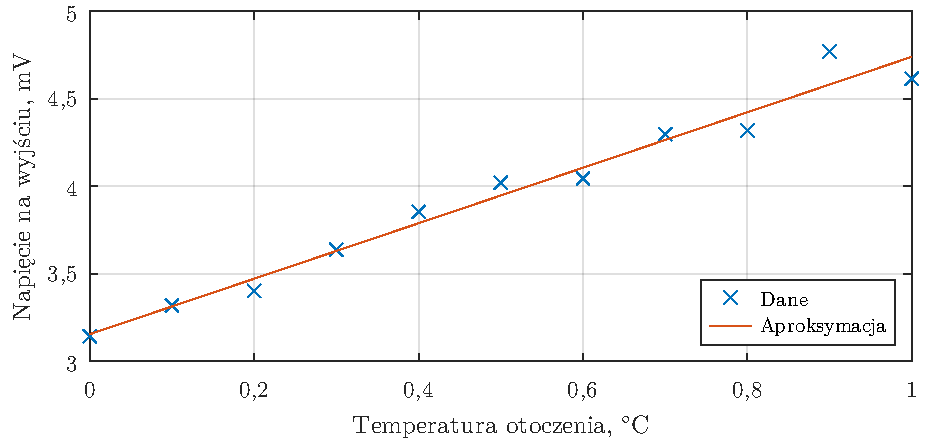
\includegraphics{plot_demo}
\makecaption{fig:octave}{Przykładowy rysunek wygenerowany w programie \texttt{GNU Octave}}
\end{figure}

Przedstawiony skrypt tworzy w pierwszej linii nowy wykres, przy czym gdy skrypt zostaje wywołany z terminala wykres ten jest ukrywany (taki zabieg ułatwia wsadowe generowanie wykresów). Następnie ustalane są wymiary wykresu (linie 5--7) oraz korygowana jest jego pozycja tak, aby wypełniał on cały obszar rysunku (linia 10). W kolejnych liniach (12--16) ustalane są parametry czcionki, przy czym z nieznanych dla autora niniejszego szablonu powodów, dla rozmiaru \qty{11}{pt} wynikowy plik cechuje się czcionką o rozmiarze \qty{12}{pt} (najprawdopodobniej występuje bliżej nieokreślony błąd w programie \texttt{GNU Octave}).

Po wygenerowaniu danych wykres jest sporządzany oraz formatowane są jego elementy. W opisach stosować można większość podstawowych funkcji \LaTeX{} do formatowania tekstu. Można również zastosować wartość \texttt{'latex'} dla opcji \texttt{'interpreter'} formatując kolejne elementy wykresu. Szczegóły opisuje \href{https://docs.octave.org/latest}{dokumentacja} programu \texttt{GNU Octave}. Znaki specjalne wstawiać można bezpośrednio w edytorze tekstu, stosując kodowanie \texttt{UTF-8}. Można także wstawiać je stosując ich nazwy, identycznie jak podczas edycji równań. Wygenerowany w omawiany sposób wykres jest spójny z resztą dokumentu i wygląda profesjonalnie.

\begin{listing}[hbt!]
\inputminted[linenos, breaklines]{octave}{skrypty/plot_demo.m}
\makecaption{lst:octave}{Przykładowy skrypt programu \texttt{GNU Octave} generujący rysunek~\ref{fig:octave}}
\end{listing}
